\documentclass[11pt]{report}
\usepackage[T1]{fontenc}
\usepackage[utf8]{inputenc}
\usepackage{graphicx}
\usepackage{hyperref}
\usepackage[explicit]{titlesec}
\usepackage{color, varwidth}
\usepackage[margin=0.75in]{geometry}
\usepackage{xhfill}
\usepackage{soul}
\graphicspath{{./images/}}

%----------------------------------------------------------------------------------------
%	SECTION HEADER STYLES
%----------------------------------------------------------------------------------------
\setlength{\headheight}{15pt}

\definecolor{darkblue}{RGB}{0,101,135}
\definecolor{ourblue}{RGB}{0,138,184}

\newcommand{\hsp}{\hspace{20pt}}
\titleformat{\chapter}[hang]{\huge\bfseries}{\thechapter\hsp\textcolor{ourblue}{|}\hsp}{0pt}{#1\Huge\bfseries}

\newcommand\Centered{%
\titleformat{\section}[hang]
  {\normalfont\large\filcenter}{}{0em}
  {\xrfill[0.3ex]{1.0pt}[ourblue]~\begin{varwidth}{.75\linewidth}\centering{\color{darkblue}##1}\end{varwidth}~\xrfill[0.3ex]{1.0pt}[ourblue]}
}

\newcommand\textline[4][t]{%
  \par\smallskip\noindent\parbox[#1]{.333\textwidth}{\raggedright#2}%
  \parbox[c]{.333\textwidth}{\centering#3}%
  \parbox[c]{.333\textwidth}{\raggedleft#4}\par\smallskip%
  \vspace{.5\baselineskip}
}

\titlespacing{\chapter}{12pt plus 4pt minus 2pt}{\parskip}{7pt}


\renewcommand\sectionmark[1]{\markboth{#1}{}}

%----------------------------------------------------------------------------------------

\begin{document}

\begin{titlepage}
\begin{center}

\newcommand{\HRule}{\rule{\linewidth}{0.5mm}}

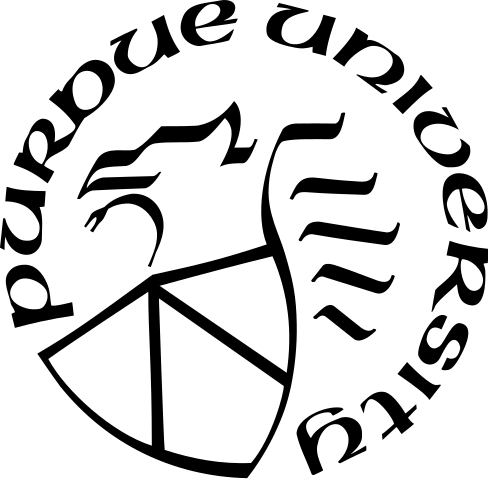
\includegraphics[width=0.25\textwidth]{purdue_seal.png}~\\[1cm]

\vspace{10mm}



\includegraphics[width=0.6\textwidth]{logo.png}~\\[1cm]

% Title
\HRule \\[0.4cm]
{ \huge \bfseries Design Document \\[0.4cm] }

\HRule \\[1.5cm]

% Author and supervisor
\noindent
\begin{minipage}{0.4\textwidth}
\begin{flushleft} \large
Abhijeet \textsc{Chakrabarti}\\
Ammar \textsc{Askar}\\
Brian \textsc{Quinn}\\
Eric \textsc{Lee}
\end{flushleft}
\end{minipage}%
\begin{minipage}{0.4\textwidth}
\begin{flushright} \large
\textsc{Team }\#29
\end{flushright}
\end{minipage}

\vfill

% Bottom of the page
{\large \today}

\end{center}
\end{titlepage}

\pagebreak

\chapter{Sprint Overview}
This sprint will most likely be the sprint that contains the heaviest workload. The main focus of this sprint is to lay the foundation for the implementation of the social networking aspect of our service. This will include giving users profiles which will eventually be implemented to communicate with other user profiles. This will also include setting up communication for users in listening rooms and finalizing the synchronous music listening features in the listening rooms. After this sprint the groundwork for social networking amongst users will be laid and music rooms should have very near complete functionality.

\begin{description}
\item[Scrum Master] Abhijeet Chakrabarti

\item[Meeting Plan] Meeting on Fridays and Saturdays in Hillenbrand

\item[Risks And Challenges] The biggest risk/challenge associated with this sprint will be the implementation of user profiles. This is due to the variable amount of features that we will try to implement for each user which may prove to be a very difficult task.
\end{description}

\chapter{Current Sprint Details}

\Centered{
    \section{User Story \#1}
}

As a user, I want to be able to listen to music simultaneously with other people.

\vspace{3mm}

\def\arraystretch{1.6}%  1 is the default, change whatever you need 
\begin{tabular}{c|c|c|c|c}
     \# & Description & Time & Team & Owner \\
     \hline
     1  & Make server tell client to play music for all users & 3 hrs & Front-End and Back-End & Eric \\
\end{tabular}

\vspace{4mm}

\subsection*{Acceptance Criteria}
\begin{itemize}
    \item \textit{Given} users are all in a listening room, \textit{when} music is playing, \textit{then} all users should be listening to the same song simultaneously.
    
\end{itemize}

\Centered{
    \section{User Story \#8}
}

As a user, I want to be able to party chat with other users in the same listening party.

\vspace{3mm}

\begin{tabular}{c|c|c|c|c}
     \# & Description & Time & Team & Owner \\
     \hline
     1  & Create a message buffer in music room model & 5 hrs & Back-End & Brian \\
     2  & Design an interface for group chat in music room page & 4 hrs & Front-End & Abhijeet\\
     3  & Let users input messages to buffer through chat UI & 4 hrs & Front-end and Back-End  & Brian\\
     4  & Display contents of message buffer in chat UI & 2 hrs & Front-End and Back-End & Brian
    
\end{tabular}

\vspace{4mm}

\subsection*{Acceptance Criteria}
\begin{itemize}
    \item \textit{Given} a user has typed a message, \textit{when} a user submits a message, \textit{then} the message should be added to a chat buffer in the music room and displayed to other users.
    
    \item \textit{Given} Messages are in the chat buffer, \textit{when}, the music room is still in session\textit{then} a history of all messages should be displayed to all users in the room.
\end{itemize}


\Centered{
    \section{User Story \#15}
}

As a user, I want to have a profile (picture, bio, favorite music, etc.)

\vspace{3mm}

\begin{tabular}{c|c|c|c|c}
     \# & Description & Time & Team & Owner \\
     \hline
     1  & Design a generic profile page template & 3 hrs & Front-End & Abhijeet \\
     2  & Add functionality to features of profile page & 8 hrs & Back-End  & Ammar \\
     3  & Implement a button to take a user to profile page & 4 hrs & Back-End & Ammar
    
\end{tabular}

\vspace{4mm}

\subsection*{Acceptance Criteria}
\begin{itemize}
    \item \textit{Given} a user is logged in, \textit{when} they click the link to display their profile, \textit{then} they should be redirected to their profile page.
    
    \item \textit{Given} a user is on their profile page, \textit{when} the user presses edit on any editable field, \textit{then} the user will be able to change the content of that field.
\end{itemize}


\Centered{
    \section{User Story \#17}
}

As a user, I want to be able to create multiple listening parties.

\vspace{3mm}

\begin{tabular}{c|c|c|c|c}
     \# & Description & Time & Team & Owner \\
     \hline
     1  & Give server ability to hold multiple music room objects & 1 hrs & Back-End & Brian\\
     2  & Add additional music rooms to server as they are created & 3 hrs & Back-End & Brian\\
\end{tabular}

\vspace{4mm}

\subsection*{Acceptance Criteria}
\begin{itemize}
    \item \textit{Given} a user wants to create an additional listening party, \textit{when} a user creates the party, \textit{then} a new music room object will be created and added to the list of rooms in the server.    
\end{itemize}



\Centered{
    \section{User Story \#20}
}

As a user, I want to be able to control the playback of the music for everyone.

\vspace{3mm}

\begin{tabular}{c|c|c|c|c}
     \# & Description & Time & Team & Owner \\
     \hline
     1  & Make client push to server when a user interacts with playback & 2 hrs & Front-End & Eric\\
     2  & Make server propagate playback instructions to all users in room & 5 hrs & Back-End  & Eric \\
\end{tabular}

\vspace{4mm}

\subsection*{Acceptance Criteria}
\begin{itemize}
    \item \textit{Given} a track is playing, \textit{when} a user presses play, pause, next, etc. , \textit{then} all users will experience the same function that one user selects.
    
\end{itemize}

\pagebreak

\chapter{Remaining Backlog}
    
    \begin{enumerate}

    \item As a user, I want to be able to listen to music simultaneously with other people.
    
    \item \st{As a user, I want to to be able to upload my own music.}
        
    \item \st{As a user, I want to be able to create an account.}
    
    \item \st{As a user, I want to be able to log in to my account.}

    \item As a user, I want to be able to have people follow my account.

    \item As a user, I want to be able to follow other users.
    
    \item As a user, I want to be able to un-follow other users.
    
    \item As a user, I want to be able to party chat with other users in the same listening party.
    
    \item As a user, I want to be able to direct message other users.
    
    \item As a user, I want to be able to invite other users to join my listening party.
    
    \item As a user, I want to be able to permanently leave certain listening parties.
    
    \item As a user, I want my followers to be able to see the recent music I have listened to.
    
    \item As a user, I want the ability to block other users. 
    
    \item As a user, I want the ability to report other users for misconduct.
    
    \item As a user, I want to have a profile (picture, bio, favorite music, etc.)
    
    \item As a user, I want to be able to set privacy settings for my account.
    
    \item As a user, I want to be able to create multiple listening parties.
    
    \item \st{As a user, I want to be able to see information about the album for playing tracks.}
    
    \item \st{As a user, I want to be able to see information about the artist for playing tracks.}

    \item As a user, I want to be able to control the playback of the music for everyone.
    
    \item As a user, I want to be able to view listener metrics and statistics.
    
    \item As an admin, I want to be able to control user accounts.
    
    \item As an admin, I want to be able to monitor usage of the service.
    
    \item As an advertiser, I want to be able to see data on people's taste in music so I can target ads to them.

\end{enumerate}

\end{document}